\documentclass[12pt]{article}
\usepackage[danish]{babel}
\usepackage{amsfonts, amssymb, mathtools, amsthm, amsmath}
\usepackage{graphicx, pgfplots}
\usepackage{url}
\usepackage[dvipsnames]{xcolor}
\usepackage{sagetex}
\usepackage{lastpage}

%loaded last
\usepackage[hidelinks]{hyperref}

\usepackage{siunitx}
  \sisetup{exponent-product = \cdot,
    output-decimal-marker = {,}}

%Giles Castelles incfig
\usepackage{import}
\usepackage{xifthen}
\usepackage{pdfpages}
\usepackage{transparent}

\newcommand{\incfig}[2][1]{%
  \def\svgwidth{#1\columnwidth}
  \import{../figures/}{#2.pdf_tex}
}

\setlength{\parindent}{0in}
\setlength{\oddsidemargin}{0in}
\setlength{\textwidth}{6.5in}
\setlength{\textheight}{8.8in}
\setlength{\topmargin}{0in}
\setlength{\headheight}{18pt}

\usepackage{fancyhdr}
\pagestyle{fancy}

\fancyhead{}
\fancyfoot{}
\fancyfoot[R]{\thepage}
\fancyhead[C]{\leftmark}

\pgfplotsset{compat=newest}

\pgfplotsset{every axis/.append style={
  axis x line=middle,    % put the x axis in the middle
  axis y line=middle,    % put the y axis in the middle
  axis line style={<->,color=black}, % arrows on the axis
}}

\usepackage{thmtools}
\usepackage{tcolorbox}
  \tcbuselibrary{skins, breakable}
  \tcbset{
    space to upper=1em,
    space to lower=1em,
  }

\theoremstyle{definition}

\newtcolorbox[auto counter]{definition}[1][]{%
  breakable,
  colframe=ForestGreen,  %frame color
  colback=ForestGreen!5, %background color
  colbacktitle=ForestGreen!25, %background color for title
  coltitle=ForestGreen!70!black,  %title color
  fonttitle=\bfseries\sffamily, %title font
  left=1em,              %space on left side in box,
  enhanced,              %more options
  frame hidden,          %hide frame
  borderline west={2pt}{0pt}{ForestGreen},  %display left line
  title=Definition \thetcbcounter: #1,
}

\newtcolorbox{greenline}{%
  breakable,
  colframe=ForestGreen,  %frame color
  colback=white,          %remove background color
  left=1em,              %space on left side in box
  enhanced,              %more options
  frame hidden,          %hide frame
  borderline west={2pt}{0pt}{ForestGreen},  %display left line
}

\newtcolorbox[auto counter, number within=section]{eks}[1][]{%
  brekable,
  colframe=NavyBlue,  %frame color
  colback=NavyBlue!5, %background color
  colbacktitle=NavyBlue!25,    %background color for title
  coltitle=NavyBlue!70!black,  %title color
  fonttitle=\bfseries\sffamily, %title font
  left=1em,            %space on left side in box,
  enhanced,            %more options
  frame hidden,        %hide frame
  borderline west={2pt}{0pt}{NavyBlue},  %display left line
  title=Eksempel \thetcbcounter: #1
}

\newtcolorbox{blueline}{%
  breakable,
  colframe=NavyBlue,     %frame color
  colback=white,         %remove background
  left=1em,              %space on left side in box,
  enhanced,              %more options
  frame hidden,          %hide frame
  borderline west={2pt}{0pt}{NavyBlue},  %display left line
}

\newtcolorbox{teo}[1][]{%
  breakable,
  colframe=RawSienna,  %frame color
  colback=RawSienna!5, %background color
  colbacktitle=RawSienna!25,    %background color for title
  coltitle=RawSienna!70!black,  %title color
  fonttitle=\bfseries\sffamily, %title font
  left=1em,              %space on left side in box,
  enhanced,              %more options
  frame hidden,          %hide frame
  borderline west={2pt}{0pt}{RawSienna},  %display left line
  title=Teori: #1,
}

\newtcolorbox[auto counter, number within=section]{sæt}[1][]{%
  breakable,
  colframe=RawSienna,  %frame color
  colback=RawSienna!5, %background color
  colbacktitle=RawSienna!25,    %background color for title
  coltitle=RawSienna!70!black,  %title color
  fonttitle=\bfseries\sffamily, %title font
  left=1em,              %space on left side in box,
  enhanced,              %more options
  frame hidden,          %hide frame
  borderline west={2pt}{0pt}{RawSienna},  %display left line
  title=Sætning \thetcbcounter: #1,
  before lower={\textbf{Bevis:}\par\vspace{0.5em}},
  colbacklower=RawSienna!25,
}

\newtcolorbox{redline}{%
  breakable,
  colframe=RawSienna,  %frame color
  colback=white,       %Remove background color
  left=1em,            %space on left side in box,
  enhanced,            %more options
  frame hidden,        %hide frame
  borderline west={2pt}{0pt}{RawSienna},  %display left line
}

\newtcolorbox{for}[1][]{%
  breakable,
  colframe=NavyBlue,  %frame color
  colback=NavyBlue!5, %background color
  colbacktitle=NavyBlue!25,    %background color for title
  coltitle=NavyBlue!70!black,  %title color
  fonttitle=\bfseries\sffamily, %title font
  left=1em,              %space on left side in box,
  enhanced,              %more options
  frame hidden,          %hide frame
  borderline west={2pt}{0pt}{NavyBlue},  %display left line
  title=Forklaring #1,
}

\newtcolorbox{bem}{%
  breakable,
  colframe=NavyBlue,  %frame color
  colback=NavyBlue!5, %background color
  colbacktitle=NavyBlue!25,    %background color for title
  coltitle=NavyBlue!70!black,  %title color
  fonttitle=\bfseries\sffamily, %title font
  left=1em,              %space on left side in box,
  enhanced,              %more options
  frame hidden,          %hide frame
  borderline west={2pt}{0pt}{NavyBlue},  %display left line
  title=Bemærkning:,
}

\makeatother
\def\@lecture{}%
\newcommand{\lecture}[3]{
  \ifthenelse{\isempty{#3}}{%
    \def\@lecture{Lecture #1}%
  }{%
    \def\@lecture{Lecture #1: #3}%
  }%
  \subsection*{\makebox[\textwidth][l]{\@lecture \hfill \normalfont\small\textsf{#2}}}
}

\makeatletter

\newcommand{\opgave}[1]{%
 \def\@opgave{#1}%
 \subsection*{Opgave #1}
}

\makeatother

%Format lim the same way in intext and in display
\let\svlim\lim\def\lim{\svlim\limits}

% horizontal rule
\newcommand\hr{
\noindent\rule[0.5ex]{\linewidth}{0.5pt}
}

\title{Eksamen i: Fysik og Mekanik}
\author{Noah Rahbek Bigum Hansen}
\date{20. januar 2021 (12. December 2024)}

\begin{document}

\maketitle

\section*{1.}
En astronaut udforsker en fjern planet, hvor tyngdeaccelerationen blot er \num{65,0}\% af hvad den er på Jorden. Han hopper af et klippefremspring \qty{500}{m} over et stort plateau. Efter \qty{5,00}{s} frit fald, aktiverer han en raketmotor (en “jet-pack”) som han har på ryggen. Herved ændres hans acceleration til en ny, konstant værdi i den tilbageværende del af faldet mod plateauet. Astronautens fødder rammer jordoverfladen (plateauet) \qty{26,0}{s} efter aktiveringen af raketmotoren. Bestem den fart hvormed han rammer jordoverfladen. (Antag at tyngdeaccelerationen på Jorden er \qty{9,80}{m / s^2}.)
\bigbreak
Tyngdeaccelerationen på den fjerne planet må være $\num{0,65}g$. Altså kan den afstand han falder i de første \qty{5,00}{s} findes vha. formlen for strækningen i et frit fald
\[ 
y = y_0 + v_{0y}t + \frac{1}{2}a_y t^2
.\]
Idet vi sætter 0-punktet til at være jorden er hans starthøjde $y_0 = \qty{500}{m}$, han starter fra stilstand og derfor er hans starthastighed $v_{0y}t = 0$. Altså har vi
\[ 
y_{5s} = \qty{500}{m} -\frac{1}{2} \num{0,65} \cdot \qty{9,80}{\frac{m}{s^2}} \cdot (\qty{5,00}{s})^2 = \qty{420,375}{m} 
.\]
Hans hastighed til dette tidspunkt kan findes vha. formlen for hastighed ved konstant acceleration
\[ 
v_{y} = v_{y0} + a_y t
.\]
Heri kan kendte størrelser indsættes for at finde astronautens hastighed efter \qty{5,00}{s} som
\[ 
v_{y5s} = 0 - \num{0,65} \cdot \qty{9,80}{\frac{m}{s^2}} \cdot \qty{5,00}{s} = \qty{-31,85}{\frac{m}{s}} 
.\]
Dermed er astronautens hastighed og position i det han tænder jet-packen kendt. Dermed kan formlen for position ved konstant acceleration igen benyttes idet den ukendte acceleration i 2. halvdel af faldet kan isoleres som
\begin{align*}
  y &= y_0 + v_{y0}t + \frac{1}{2}a_y t^2 \\
  \frac{1}{2}a_y t^2 &= y - y_0 - v_{y0}t \\
  a_y &= 2\cdot \frac{y - y_0 - v_{y0}t}{t^2}
.\end{align*}
Idet astronautens slutposition $y = 0$, startposition $y_0 = y_{5s} = \qty{420,375}{m}$, starthastighed $v_{y0} = v_{y5s} = - \qty{31,85}{\frac{m}{s}}$ og tiden før han rammer jorden $t = \qty{26,0}{s}$ alle er kendte kan accelerationen i den sidste halvdel af faldet findes som
\[ 
a_y = 2\cdot \frac{- \qty{420,375}{m} + \qty{31,85}{\frac{m}{s}} \cdot \qty{26,0}{s}}{(\qty{26,0}{s})^2 } = \qty{1,206}{\frac{m}{s^2}} 
.\]
Altså er astronautens nye konstante acceleration efter han tænder jet-packen $a_y = \qty{1,206}{\frac{m}{s^2}}$. Denne kan indsættes i formlen for hastighed ved konstant acceleration, som også blev brugt ovenfor, som
\[ 
  v_y = v_{y0} + a_y t \implies v_y = -\qty{31,85}{\frac{m}{s}} + \qty{1,206}{\frac{m}{s^2}} \cdot \qty{26,0}{s} = \qty{-0,494}{\frac{m}{s}} 
.\]
Altså rammer astronauten jorden med en hastighed på \qty{0,494}{m \per s} med retning mod jorden.

\section*{2.}
\begin{figure} [ht]
  \centering
  \caption{}
  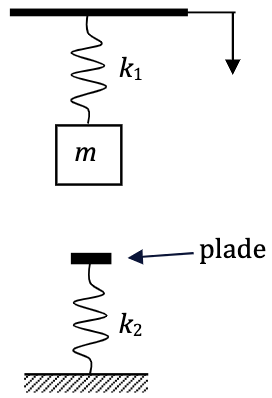
\includegraphics[width=0.25\linewidth]{../figures/Ek21_1.png}
  \label{fig:Ek21_1}
\end{figure}

Et legeme med massen $m = \qty{5,00}{kg} $ hænger i en masseløs fjeder, som vist i \textbf{\autoref{fig:Ek21_1}}. Nedenfor er der en plade, monteret på en anden fjeder. Når massen $m$ ikke rører pladen (se igen \textbf{\autoref{fig:Ek21_1}}), er den øverste fjeder strakt \qty{490}{mm}  (relativt til fjederens naturlige længde).

\subsection*{(a)}
Bestem fjederkonstanten $k_1$ (I enheden \unit{N/m}) for den øverste fjeder. (Antag at tyngdeaccelerationen $g = \qty{9,80}{\frac{m}{s^2}}$.)
\bigbreak
Den eneste kraft der virker på den øverste fjeder er massen $m$'s tyngde. Altså må det, idet det antages, at der er statik, gælde, at fjederkraften fra den øverste fjeder netop svarer til kassens tyngde. Altså har vi
\begin{align*}
  w &= F \\
  mg &= k_1x \\
  k_1 &= \frac{mg}{x} \\
  &= \frac{\qty{5,00}{kg} \cdot \qty{9,80}{\frac{m}{s^2}}}{\qty{0,49}{m}} \\
  &= \qty{100}{\frac{N}{m}}  \\
.\end{align*}
Altså er fjederkonstanten $k_1 = \qty{100}{\frac{N}{m}}$. 


\subsection*{(b)}
Massen $m$ sænkes nu langsomt ned, sådan at den hviler på pladen, og sådan at den øverste fjeder strækkes blot \qty{400}{mm} (igen, relativt til fjederens naturlige længde). Herved sammentrykkes den nederste fjeder \qty{30,0}{mm}. Bestem fjederkonstanten $k_2$ (igen i enheden \unit{N/m}) for den nederste fjeder.
\bigbreak
For at der er statik gælder at
\[ 
F_2 - w + F_1 = 0 \implies F_2 = w - F_1
.\]
Kraften fra den øverste fjeder, $F_1$, kan findes vha. formlen for kraften i en fjeder, også brugt ovenfor, som
\[ 
F_1 = k_1 \cdot x_1 = \qty{100}{\frac{N}{m}} \cdot \qty{0,400}{m} = \qty{40,0}{N} 
.\]
Vi har dermed at
\[ 
F_2 = \qty{49,0}{N} - \qty{40,0}{N} = \qty{9,00}{N} 
.\]
Og dermed kan fjederkonstanten $k_2$ findes som
\[ 
k_2 = \frac{F_2}{x_2} = \frac{\qty{9,00}{N}}{\qty{0,0300}{m}} = \qty{300}{\frac{N}{m}} 
.\]




\subsection*{(c)}
Massen $m$ sænkes langsomt yderligere ned. Hvor meget sammentrykkes den nederste fjeder i det øjeblik den øverste fjeder er ustrakt?
\bigbreak
Idet den øverste fjeder er ustrakt må den nederste fjeder skulle udøve en kraft der netop modsvarer kassens tyngde. Altså 
\begin{align*}
  F_2 &= w \\
  k_2x_2 &= mg \\
  x_2 &= \frac{mg}{k_2} \\
  &= \frac{\qty{5,00}{kg} \cdot \qty{9,80}{\frac{m}{s^2}} }{\qty{300}{\frac{N}{m}} } \\
  &= \qty{0,163}{m} = \qty{16,3}{cm}
.\end{align*}
Altså vil den nederste fjeder blive sammenpresset i alt \qty{16,3}{cm} under de givne forhold.

\section*{3.}
\begin{figure} [ht]
  \centering
  \caption{}
  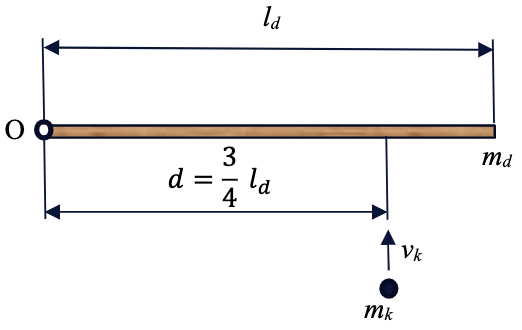
\includegraphics[width=0.4\linewidth]{../figures/Ek_21_2.png}
  \label{fig:Ek_21_2}
\end{figure}

En dør med bredden $l_d$ og massen $m_d$ er i hvile, hvorefter den rammes af en klump ler med massen $m_k$, som bevæger sig med farten $v_k$ i det øjeblik den rammer døren (se \textbf{\autoref{fig:Ek_21_2}}). Døren rammes i afstanden $d = \frac{3}{4}l_d$ fra rotationsaksen (d.v.s. fra hængslet). Lerklumpen rammer vinkelret på døren og bliver siddende efter anslaget.

\subsection*{(a)}
Vis at dørens inertimoment (``moment of inertia'') omkring omdrejningspunktet $O$ er givet ved $I_0 = \frac{1}{3} m_dl_d^2$.
\bigbreak
Inertimomentet kan generelt findes som
\[ 
I = \int x^2 \, \mathrm{d}m
.\]
Altså skal et udtryk for $\mathrm{d}m$ findes. For en tynd rektangulær plade med masse $M$, bredde $l_d$ og højde $h$ er massen pr. areal givet som
\[ 
\sigma = \frac{m_d}{l_dh}
.\]
Arealet af en tynd stribe med tykkelse $\mathrm{d}x$ og en afstand $l$ til origo er da
\[ 
A = h \, \mathrm{d}x
.\]
Massen af denne tynde stribe bliver da
\[ 
\mathrm{d}m = \sigma A = \frac{m_d}{l_dh} h \, \mathrm{d}x = \frac{m_d}{l_d} \, \mathrm{d}x 
.\]
Dette sættes ind i integralet fra før som
\begin{align*}
  I_0 &= \int_0^{l_d} x^2 \frac{m_d}{l_d} \, \mathrm{d}x  \\
    &= \frac{m_d}{l_d} \int_0^{l} x^2 \, \mathrm{d}x \\
    &= \frac{m_d}{l:d} \frac{1}{3}l^3 \\
    &= \frac{1}{3}m_dl_d^2
.\end{align*}
Altså er det vist. 


\subsection*{(b)}
Bestem dør-lerklump systemets vinkelhastighed $\omega$ umiddelbart efter lerklumpens anslag mod døren. (Bemærk at lerklumpens masse $m_k$ \textit{ikke} kan ignoreres. Derimod kan der ses bort fra friktion i hængslet $O$.)
\bigbreak
Idet lerklumpen antages at være en punktmasse har den ikke et inertimoment omkring sin egen omdrejningsakse. Dog har den fra parallel-akse-teoremet et inertimoment på 
\[ 
I = md^2 \implies I_k = m_k \cdot \frac{9}{16} \cdot l_d^2
.\]
Det samlede inertimoment for 
systemet bliver derfor
\[ 
I = I_0 + I_k = \frac{1}{3} m_d l_d^2 + m_k \cdot \frac{9}{16} l_d^2 = l_d^2 \left( \frac{1}{3}m_d + \frac{9}{16}m_k \right)
.\]
Konservation af impulsmoment giver at
\[ 
I \cdot \omega - m_k v_k d = 0
.\]
Dette kan omskrives til
\begin{align*}
  I \cdot \omega &= m_k v_k d \\
  l_d^2 \left( \frac{1}{3}m_d + \frac{9}{16}m_k \right) \omega &= m_k v_k \cdot \frac{3}{4}l_d  \\
  \omega &= \frac{3}{4l_d^2} \cdot \frac{m_k v_k l_d}{\frac{1}{3}m_d + \frac{9}{16}m_k} \\
  &= \frac{3}{4l_d}\cdot \frac{m_k v_k}{\frac{1}{3} m_d + \frac{9}{16}m_k} \\
  &= \frac{9}{4l_d} \cdot \frac{m_k v_k}{ m_d + \frac{27}{16}m_k} \\
  &= \frac{36}{l_d} \cdot \frac{m_k v_k}{16 m_d + 27 m_k}
.\end{align*}



\section*{4.}
Denne opgave omhandler effektiviteten af en totrinsraket, sammenholdt med effektiviteten af en “ettrinsraket” (d.v.s. en raket med blot et enkelt raketmotor-trin).


\subsection*{(a)}
\begin{figure} [ht]
  \centering
  \caption{}
  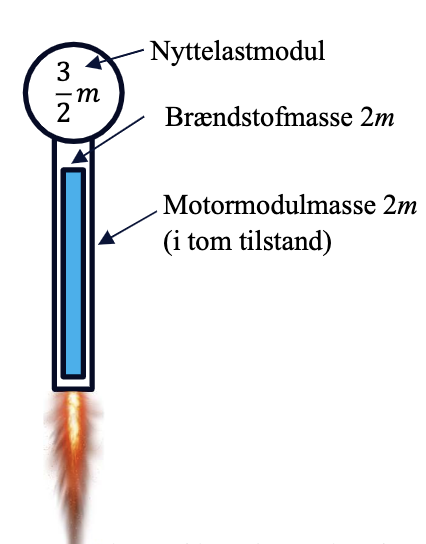
\includegraphics[width=0.15\linewidth]{../figures/Ek21_3.png}
  \label{fig:Ek21_3}
\end{figure}

Betragt først en ettrinsraket, bestående af et nyttelastmodul (“payload module”) med massen $\frac{3}{2}m$ og et motormodul, som også indeholder brændstoffet. Det tomme motormodul har massen $2m$. Det indeholdte brændstof har ligeledes massen $2m$. (Se \textbf{\autoref{fig:Ek21_3}}) Rakettens samlede masse, med fuld brændstoftank, er således $\frac{11}{2}m$. Til at begynde med er raketten i hvile, langt ude i “det ydre rum”, fjernt fra nogen planet. Det antages at al brændstoffet (d.v.s. massen $2m$) nu antændes og udstødes, øjeblikkeligt og samtidigt, med hastigheden $\Vec{v}_{\text{fuel}}$. Bestem den hastighed som nyttelastmodulet og det tomme motormodul opnår herved, udtrykt ved hastigheden $\Vec{v}_{\text{fuel}}$.
\bigbreak
Der er i opgaven givet massen af nyttelastmodulet $m_{\text{pl}} = \frac{3}{2}m$, massen af mototren $m_{\text{m-mot}} = 2m$, massen af brændstoffet $m_{\text{fuel}} = 2m$ og den totale masse af den fulde raket $m_{\text{tot-f}} = m_{pl} + m_{mot} + m_{fuel} = \frac{11}{2}m$. Desuden har vi fra impulsbevarelse at
\[ 
\Vec{p}_0 = 0; \qquad \Vec{p}_1 = \Vec{p}_{raket} + \Vec{p}_{fuel} = \Vec{p}_0 = 0
.\]
Altså må det gælde at impulsen på den udstødte brændstof netop tilsvarer impulsen for raketten, dog i modsat retning, som
\[ 
\Vec{p}_{raket} = \Vec{-p}_{fuel} \implies p_{raket} = p_{fuel}
.\]
Hvor $p_{raket} = |\Vec{p}_{raket}|$ og $p_{fuel} = |\Vec{p}_{fuel}|$. Det ovenstående omskrives til
\[ 
  m_{tot-e} \cdot v_{tot-e} = m_{fuel} \cdot v_{fuel} \implies v_{tot-e} = \frac{m_{fuel} \cdot v_{fuel}}{m_{tot-e}}
.\]
Vi har desuden at $m_{tot-e} = m_{tot-f} - m_{fuel} = \frac{7}{2}m$. Vi får da
\[ 
v_{tot-e} = \frac{2m v_{fuel}}{\frac{7}{2}m} = \frac{4}{7} v_{fuel}
.\]
Og idet retningerne igen regnes ind bliver det endelige udtryk for $\Vec{v}_{tot-e}$ at
\[ 
\Vec{v}_{tot-e} = -\frac{4}{7} \Vec{v}_{fuel}
.\]



\subsection*{(b)}
\begin{figure} [ht]
  \centering
  \caption{}
  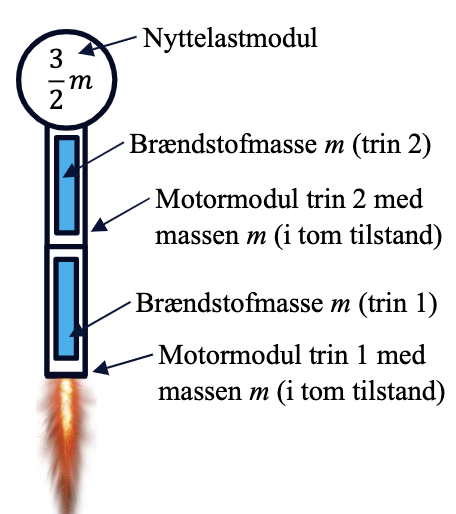
\includegraphics[width=0.15\linewidth]{../figures/Ek21_4.png}
  \label{fig:Ek21_4}
\end{figure}

Betragt dernæst en totrinsraket, som vist i \textbf{\autoref{fig:Ek21_4}}. Nyttelastmodulet har igen massen $\frac{3}{2}m$, men nu der der to motormoduler, d.v.s. to trin, der hver især indeholder brændstof med massen $m$ (se igen \textbf{\autoref{fig:Ek21_4}}). Rakettens samlede masse, med fyldte brændstoftanke, er således igen $\frac{11}{2}m$, præcis som  før.  Begge  trin  udstøder  brændstof  med  hastigheden $\Vec{v}_{\text{fuel}} = \Vec{v}_{\text{ex}} + \Vec{v}_{\text{i}}$, hvor $\Vec{v}_{\text{ex}}$ er udstødningshastigheden relativt til raketten, og $\Vec{v}_{i}$ er rakettens hastighed i det øjeblik brændstoffet er opbrugt. Igen antages det at raketten til at begynde med er i hvile. Så antændes brændstoffet i trin 1, og det hele (d.v.s. hele massen $m$) udstødes øjeblikkeligt. Dernæst afkobles det tomme motormodul, trin 1, fra den resterende del af raketten, og brændstoffet i trin 2 antændes og udstødes (igen, hele massen $m$ på én gang, øjeblikkeligt). Bestem sluthastigheden for nyttelastmodulet og det tilkoblede, tomme motormodul, trin 2, og konkluder hvilket raketdesign der ultimativt giver nyttelastmodulet den største fart. (Vink: Bestem rakettens hastighed efter affyring af trin 1. Eftersom det tomme trin 1 nu afkobles, er det fordelagtigt derefter at redefinere systemet til at bestå af blot nyttelastmodulet samt trin 2.)
\bigbreak
Vi har oplyst, at massen af nyttelastmodulet $m_{nytte} = \frac{3}{2}m$, massen af hvert brændstoftrin $m_{fuel} = m$, massen af begge motorer $m_{mot} = m$ og udstødninghastigheden $\Vec{v}_{ex}$. Vi har igen impulskonservation så det gælder at
\[ 
 \ \Vec{p}_1 = \Vec{p}_{raket} + \Vec{p}_{fuel} = \Vec{p}_0 = 0
.\]
Hvilket igen giver 
\[ 
\Vec{p}_{raket} = -\Vec{p}_{fuel} \implies p_{raket} = p_{fuel}
.\]
Hvor $p_{raket} = |\Vec{p}_{raket}|$ og $p_{fuel} = |\Vec{p}_{fuel}|$. Det ovenstående kan omskrives til
\[ 
  (m_{nytte} + m_{fuel} + 2m_{mot}) \cdot v_{1} = m_{fuel} \cdot v_{ex} \implies v_1 = \frac{m_{fuel}\cdot v_{ex}}{m_{nytte} + m_{fuel} + 2m_{mot}} 
.\]
Sættes de givne størrelser ind kan hastigheden af rakketten før første motor frakobles findes til
\[ 
v_1 = \frac{mv_{ex}}{\frac{3}{2}m  + m+ 2m} = \frac{2}{9} v_{ex} \implies \Vec{v}_1 = - \frac{2}{9}v_{ex}
.\]
Herefter frakobles det ene motormodul og det andet brændstoftrin antændes. Dermed bliver impulskonservationen
\[ 
\Vec{p}_1 = \Vec{p}_2 \implies (m_{nytte} + m_{mot} + m_{fuel})\cdot v_1 = (m_{nytte} + m_{mot})v_2 + m_{fuel}v_{fuel}
.\]
Heri isoleres sluthastigheden, $v_2$ som
\begin{align*}
  v_2 &= \frac{(m_{nytte} + m_{tot} + m_{fuel}) \cdot v_1 - m_{fuel}\cdot v_{fuel}}{m_{nytte} + m_{mot}} \\
      &= \frac{\left( \frac{3}{2}m + m + m \right)\cdot \left(-\frac{2}{9} \right)v_{ex} - m \cdot \left( v_{ex} -\frac{2}{9} v_{ex} \right)}{\frac{3}{2}m + m} \\
&= \frac{\frac{7}{2}m \cdot \left( -\frac{2}{9} \right)v_{ex} - m \cdot \frac{7}{9}v_{ex}}{\frac{5}{2}m} \\
&=\frac{\frac{7}{2} \cdot -\frac{2}{9} v_{ex} - \frac{7}{9}v_{e x}}{\frac{5}{2}} \\
&= \frac{2}{5} \cdot \left( -\frac{7}{9} - \frac{7}{9} \right)v_{ex} \\
&= \frac{2}{5} \cdot -\frac{14}{9} v_{ex} \\
&= -\frac{28}{45}v_{ex}
.\end{align*}
Altså er $v_1 \approx \num{0,57} < v_2 \approx \num{0,62}$. D.v.s. to-trins-raketten er den mest effektive.


\end{document}
